\newpage
\begin{center}
	\textbf{\large 1. СРЕДНЕ-ДИСПЕРСИОННЫЙ АНАЛИЗ ПОРТФЕЛЯ}
\end{center}
\refstepcounter{chapter}
\addcontentsline{toc}{chapter}{1. СРЕДНЕ-ДИСПЕРСИОННЫЙ АНАЛИЗ ПОРТФЕЛЯ}

В этой главе определяеются основные понятия инвестирования и средне-дисперсионного анализа.
Формулируется задача поиска оптимального портфеля.

\section{Основные понятия}

Портфельный анализ берет свое начало с выхода статьи Гарри Марковица в 1952 г \cite{markowitz}. Подход Марковица начинается с предположения что инвестор в 
настоящий момент времени имеет конкретную сумму денег для инвестирования. Эти деньги будут инвестированы на определенный промежуток
времени, который назывется \textbf{периодом инвестирования}. В конце периода инвестор продает активы купленные в
ранее. 
Набор приобретенных активов иначе называют \textbf{инвестиционным портфелем}. Поэтому проблема выбора и распределения
средств по активам имеет название \textbf{проблемой выбора инвестиционного портфеля}.

Пусть цены актива на начало и конец периода инвестирования равны $S^0$ и $S^1$ соотвественно.
Определим \textbf{доходность актива} (Return) $r$ за период инвестирования как
\[
\label{eq:ROI}
	r = \frac{S^1 - S^0}{S^0}
\]

При формировании портфеля в начальный момент времени, инвестор должен иметь в виду, что доходность активов
за будущий период владения заранее не известна. То есть, он вынужден принимает решение о выборе портфеля исходя из 
своих ожидаемых доходностей активов. 

Если инвестор ставит задачей максимизировать доходность портфеля, то в этом случае его портфель должен состоять из единственного
актива с наибольшей ожидаемой доходностью. Марковиц отмечает, что такой подход не является разумны, потому что типичный инвестор
хоть и желает чтобы <<доходность была высокой>>, но одновременно требует чтобы <<доходность была настолько определенной насколько
это возможно>>. Это означает, что инвестор, стремясь одновременно максимизировать доходность и минимизировать риск 
(неопределенность), имеет две противоречащие друг другу цели. Подход Марковиа к принятию решения дает возможность адекватно 
учесть обе эти цели.

Имея $N$ доступных активов можно сформировать бесконечно много портфелей. Это множество называют \textbf{достижимым}. 
Как инвестору в этих условиях выбрать портфель? Логичными являются следующие принципы при формировании портфеля:
\begin{itemize}
	\item Из двух портфелей с одинаковым риском, инвестор выберет порфтель с большей ожидаемой доходностью
	\item Из двух портфелей с одинаковой доходностью, инвестор выберет портфель с меньшим риском
\end{itemize}
Другими словами, из достижимого множества портфелей инвестор склонен выбирать парето-оптимальные портфели.
Множество оптимальных портфелей иначе называют \textbf{эффективным множеством}. Достижимые портфели не из 
эффективного множества называют \textbf{неэффективными портфелями}.

Вопрос выбора конкретного портфеля из эффективного множества остается на стороне инвестора. Здесь он уже руководствуется
своей внутренней толерантностю к риску. Обычно достаточно зафиксировать приемлимый уровень риска внутри достижимого множества
и выбрать портфель с соответсвующей доходностью. 


\section{Постановка задачи поиска оптимального портфеля}

Будем рассматривать одношаговую задачу инвестирования. Инвестор собирает портфель по рыночным ценам активов $S^0$
стоимостью $x$ в момент времени $n=0$, а момент времени $n=1$ этот портфель продается по рыночным ценам $S^1$.

Пусть инветору доступно инвестирование в $N$ активов и начальный капитал $x$. 
Цены активов в начальный момент времени $n=0$ равны
$S_1^0, \dots, S_N^0$

Обзначим 
\begin{align}
	b = (b_1, \dots, b_N), b_i \ge 0
\end{align}
$i=\overline{1, N}$ число активов которые преобрел инвестор.

Тогда стоимость портфеля в начальный момент времени равна
\begin{align}
	X^0 = b_1 S_1^0 + \dots + B_N S_N^0
\end{align}

Иначе говоря, $b$ есть портфель ценных бумаг, где $b_i$ -- число $i$-х акций, приобретенных по цене $S_i^0$.

Будущие цены акций в момент времени $n=1$ равны $S_1^1, \dots, S_N^1$. 
Их можно представить в терминах доходностей $r_i$ используя начальные цены
\begin{align}
	S_i^1 = (1 + r_i) S_i^0, i=\overline{1, N}
\end{align}

Здесь $r_i$ являются случайными величинами.


Если инвестор cформировал портфель $b = (b_1, \dots, b_N )$, то его начальный капитал $X^0 = x$ превратится в 
\begin{align}
	X^1 = b_1 S_1^1 + \dots + b_N S_N^1,
\end{align}

Таким образом, стоимость портфеля на конец периода инвестирования является случайной величиной. 
Она определяется набором случайных величин --- будущими доходностями активов, и тем как инвестор распределил капитал
по доступным актвам. Если на первое повлиять невозможно, то второе полностью определяется инвестором.
В его интересах собрать такой портфель, цена которого будет <<побольше>> и с высокой уверенностью.
Это стремление максимизировать прибыть и минимизировать риск (неопределенность), Марковиц формулирует в терминах
математического ожидания $\E{X^1}$ и дисперсии $\D{X^1}$ случайной величины $X^1$.

Имея эти две характеристики, можно по-разному формулировать оптимизационную задачу выбора наилучшего портфеля в
зависимости от критерия оптимальности.

Можно, например, задаться вопросом о том, на каком портфеле $b^*$ достигается максимум некоторой целевой функции 
$f = f(\E{X^1}, \D{X^1})$ при <<бюджетном ограничении>> на класс допустимых портфелей:
\begin{align}
	B(x) = \{b=(b_1, \dots, b_N): b_i \ge 0, X_0(b) = x\}, x > 0
\end{align}

Задача, сформулированная в этом разделе, допускает записи в более удобном виде. А именно, перейти от абсолютных цен
к доходностям.

\section{Сведение к доходностям}

Сформулированная задача позволяет рабоать не с будущими ценами активов $S_1^1, \dots, S_N^1$,
а с доходностями $r_1, \dots, r_N$.

Перейдем от величин $b = (b_1, \dots, b_N)$ к величинам $\omega = (\omega_1, \dots, \omega_N)$, которые определим как
\begin{align}
	\omega_i = \frac{b_i S_i^0}{x}
\end{align}
причем $\omega_i \ge 0, i=\overline{1, N}$ и
\begin{align}
	\sum_{i=1}^{N} \omega_i 
	= \sum_{i=1}^{N} \frac{b_i S_i^0}{x}
	= \frac{1}{x} \sum_{i=1}^{N} b_i S_i^0
	= \frac{X^0}{x} = 1
\end{align}
Таким образом, $\omega$ есть не что иное как доли капитала, инвестируемые в соответсвующие активы.

Рассмотрим цену портфеля в момент времени $n=1$. Доходность всего портфеля обозначим через $R$. Тогда
\begin{align}
	X^1 = (1 + R) X^0
\end{align}

\begin{align}
	R &= \frac{X^1}{X^0} - 1 
	= \frac{X^1}{x} - 1 
	= \left(\frac{\sum_{i=1}^{N}b_i S_i^0}{x}\right) - 1 
	= \left(\sum_{i=1}^{N} \omega_i \frac{S_i^1}{S_i^0}\right) - 1 = \\
	&= \left(\sum_{i=1}^{N} \omega_i \frac{S_i^1}{S_i^0}\right) - \sum_{i=1}^{N} \omega_i
	= \sum_{i=1}^{N} \omega_i \frac{S_i^1}{S_i^0} - \omega_i 
	= \sum_{i=1}^{N} \omega_i \left(\frac{S_i^1}{S_i^0} - 1\right) = \\
	&= \sum_{i=1}^{N} \omega_i r_i
\end{align}

Доходность всего портфеля определяется как смесь случайных величин --- доходностей активов
входящих в портфель.

\begin{align} \label{eq:ER}
	\E{R} = \E{\sum_{i=1}^{N} \omega_i r_i} 
	= \sum_{i=1}^{N} \omega_i \E{r_i}
\end{align}

\begin{align} \label{eq:DR}
	\D{R} = \D{\sum_{i=1}^{N} \omega_i r_i} 
	= \sum_{i=1}^{N} \omega_i^2 \D{r_i} 
	+ \sum_{i=1, j=1, i \ne j}^{N} \omega_i \omega_j \COV{r_i}{r_j}
\end{align}

Уравнения \ref{eq:ER} и \ref{eq:DR} удобно переписать в матричном виде. 

Пусть 
\begin{align}
	r = (r_1, \dots, r_N) \in \R^N
\end{align}
--- вектор-столбец доходностей активов (случайный вектор).

Математическое ожидание доходностей
\begin{align}
	\mu = \E{r} = \left(\E{r_1}, \dots, \E{r_N}\right)	
\end{align}
и матрица ковариаций
\begin{align}
	\Sigma = \left\{\sigma_{ij} = \COV{r_i}{r_j}\right\}_{i=1, j=1}^{N, N} \in \R^{N \times N}
\end{align}
распределение капитала по активам
\begin{align}
	\omega = \left(\omega_1, \dots, \omega_N \right) \in \R^N
\end{align}

Доходность портфеля (случайная величина) есть
\begin{align}
	R = \omega^T r
\end{align}

Математическое ожидание доходности портфеля обозначим $\mu_X$
\begin{align}
	\mu_X = \E{R} = \E{\omega^T r} = \omega^T \mu
\end{align}

а дисперсию $\sigma_X^2$
\begin{align}
	\sigma_X^2 = \D{R} = \D{\omega^T r} = \omega^T \Sigma \omega
\end{align}

Полученные матричные обозначения позволяют удобно сформулировать задачу оптимизации.
Причем эту задачу можно ставить в различных постановках.

\section{Оптимизационная задача}

Предположим, что нам известны математические ожидания $\mu$ и ковариации $\Sigma$ доходностей активов за период инвестирования.
На практике, конечно же, эти величины не известны и их приходится оценивать. Но в этом пункте сфокусируемся
на постановке и решении оптимизационной задачи при извесных входных данных.

Для удобства матричных записей используется обозначение $e = (1, \cdots, 1) \in \R^N$ --- единичный вектор-столбец.


В качестве целевой функции возьмем линейную комбинацию доходности и риска портфеля. Для этого введем риск-параметр $\tau$.
\begin{align}
	f\left(\mu_X, \sigma_X^2 \right) = \tau \omega^T \Sigma \omega - \omega^T \mu \rightarrow \min_{\omega}
\end{align}

Используя риск-параметр $\tau \in [0, +\infty]$, оптимизационную задачу можно сформулировать в следующем виде
\begin{align}
	\begin{cases}
		\tau \omega^T \Sigma \omega - \omega^T \mu \rightarrow \min_{\omega} \\
		\omega^T e = 1 \\
		\omega \ge 0
	\end{cases}
\end{align}

Множество решений при различных значениях $\tau$ образуют эффективное множество портфелей.
При $\tau = 0$ имеем портфель минимального риска.

Альтернативно можно записать оптимизационную задачу когда риск портфеля нужно зафиксировать на определенном уровне
\begin{align}
	\begin{cases}
		-\omega^T \mu \rightarrow \min_{\omega} \\
		\omega^T \Sigma \omega \le \sigma_X^2 \\
		\omega^T e = 1 \\
		\omega \ge 0
	\end{cases}
\end{align}

Аналогично, если требуется зафиксировать определенную доходность
\begin{align}
	\begin{cases}
		\omega^T \Sigma \omega \rightarrow \min_{\omega} \\
		\omega^T \mu \ge \mu_X \\
		\omega^T e = 1 \\
		\omega \ge 0
	\end{cases}
\end{align}

% \begin{figure}[H]
% 	\centering
% 	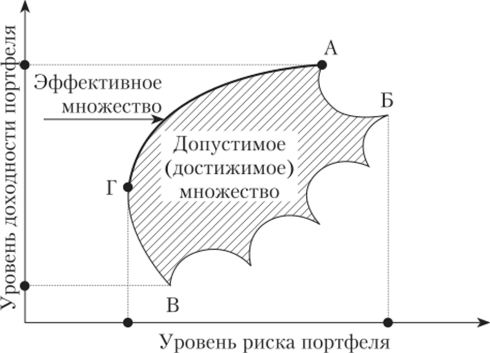
\includegraphics[width=\textwidth]{port_set.png}
% 	\caption{Множество портфелей}
% 	\label{fig:port_set}
% \end{figure}

Полученные задачи решаются с помощью хорошо изученных методов квадратичного программирования.

Конечно, на практике распределения будущих доходностей, или хотябы их характрестики неизвестны.
Поэтому для применения портфельной теории требуется оценить среднее и коварицию будущих доходностей.
На основани истории наблюдений за доходностями активов можно построить прогноз необходимых характеристик
и решать оптимизационную задачу.

Еще одним важным понятием в портфельной теории является диверсификация. Прежде чем переходить к рассмотрению методов оценки
будущих доходностей, рассмотрим как с помощью диверсификации можно редуцировать риск портфеля.

\section{Диверсификация портфеля}

Обратимся теперь к вопросу о том, как диверсификацией можно добится снижения риска, измеряемого дисперсией
или стандарным отклонением величины $R$.

С этой целью рассмотрим для начала пару случайных величин $\xi_1$ и $\xi_2$ с конечными вторыми моментами. Тогда если $c_1$ и $c_2$ -- константы,
$\sigma_i = \sqrt{\D{\xi_i}}, i=1,2$, то 
\begin{align}
\D{c_1 \xi_1 + c_2 \xi_2} = 
	(c_1 \sigma_1 - c_2 \sigma_2)^2 + 2 c_1 c_2 \sigma_1 \sigma_2 (1 + \sigma_{12}),
\end{align}
где $\sigma_{12} = \frac{\COV{\xi_1}{\xi_2}}{\sigma_1 \sigma_2}, \COV{\xi_1}{\xi_2} = \E{\xi_1 \xi_2} - \E{\xi_1} \cdot \E{\xi_2}$.
Отсюда ясно, что если $c_1 \sigma_1 = c_2 \sigma_2$ и $\sigma_{12} = -1$, то $\D{c_1 \xi_1 + c_2 \xi_2} = 0$.

Таким образом, если величины $\xi_1$ и $\xi_2$ отрицательно коррелированы с коэффициентом корреляции $\sigma_{12} = -1$, то таким подбором
констант $c_1$ и $c_2$, что $c_1 \sigma_1 = c_2 \sigma_2$, получаем комбинацию $c_1 \xi_1 + c_2 \xi_2$ с нулевой дисперсией. Но,
конечно, при этом среднее значение $\E{c_1 \xi_1 + c_2 \xi_2}$ может оказаться достаточно малым. (Случай $c_1 = c_2 = 0$ для задачи 
оптимизации не интересен в силу условия $b \in B(X))$.

Из этих элементарных рассуждений ясно, что при заданных ограничениях на $(c_1, c_2)$ и класс величин $(\xi_1, \xi_2)$ при решении задачи о том,
чтобы сделать $\E{c_1 \xi_1 + c_2 \xi_2}$ <<побольше>>, а $\D{c_1 \xi_1 + c_2 \xi_2}$ <<поменьше>>, надо стремиться к выбору таких пар 
$(\xi_1, \xi_2)$, для которых их ковариация была бы как можно ближе к минус единице.

Изложенный эффект отрицательной коррелированности, называемый эффектом Марковица, является одной из основных идей диверсификации при инвестировании ---
при составлении портфеля ценных бумаг надо стремиться к тому, чтобы вложения делались в бумаги, среди которых по возможности много отрицательно коррелированных.

Другая идея, лежащая в основе диверсификации, основана на следующем соображении.

Пусть $\xi_1, \dots, \xi_N$ --- последоватльность некоррелированных случайных величин с дисперсиями $\D{\xi_i} \le C, i=1, \dots, N$, 
где $C$ --- некоторая константа. Тогда
\begin{align}
\D{\omega_1 \xi_1 + \dots + \omega_N \xi_N} = \sum_{i=1}^{N} \omega_i^2 \D{\xi_i} \le C \sum_{i=1}^{N} \omega_i^2 .
\end{align}

Поэтому, взяв, например, $\omega_i = \frac{1}{N}$, находим, что
\begin{align}
\D{\omega_1 \xi_1 + \dots + \omega_N \xi_N} \le \frac{C}{N} \rightarrow 0, N \rightarrow \infty
\end{align}

Этот эффект некоррелиованности говорит о том, что если инвестирование производится в некоррелированные ценные бумаги, то для уменьшения риска
$\D{\omega_1 \xi_1 + \dots + \omega_N \xi_N}$, надо по возможности брать их число $N$ как можно большим.

Вернемся к вопросу о дисперсии $\D{R}$ величины
\begin{align}
	R = \omega_1 r_1 + \dots + \omega_N r_N
\end{align}

Имеем
\begin{align}
	\D{R} = \sum_{i=1}^{N} \omega_i^2 \D{r_i} + \sum_{i, j = 1, i \ne j}^{N} \omega_i \omega_j \COV{r_i}{r_j}
\end{align}

Возьмем здесь $\omega_i = \frac{1}{N}$. Тогда
\begin{align}
	\sum_{i=1}^{N} \omega_i^2 \D{r_i}
	&= \sum_{i=1}^{N} \frac{1}{N^2} \D{r_i}
	= \frac{1}{N^2} \sum_{i=1}^{N} \D{r_i}
	= \frac{1}{N} \cdot \frac{1}{N} \sum_{i=1}^{N} \D{r_i} = \\
	&= \frac{1}{N} \cdot \overline{\sigma}_N^2 ,
\end{align}
где $\bar{\sigma}_N^2 = \frac{1}{N} \sum_{i=1}^{N} \D{r_i}$ --- средняя дисперсия. 

Далее,
\begin{align}
	\sum_{i, j = 1, i \ne j}^{N} \omega_i \omega_j \COV{r_i}{r_j}
	&= \frac{1}{N^2} \cdot \sum_{i, j = 1, i \ne j}^{N} \COV{r_i}{r_j} = \\
	&= \frac{1}{N^2} \cdot N (N-1) \cdot \frac{1}{N (N-1)} \sum_{i, j = 1, i \ne j}^{N} \COV{r_i}{r_j} = \\
	&= \frac{N-1}{N} \cdot \overline{\Cov}_N
\end{align}
где $\overline{\Cov}_N$ есть средняя ковариация
\begin{align}
\overline{\Cov}_N = \frac{1}{N (N - 1)} \sum_{i, j = 1, i \ne j}^{N} \COV{r_i}{r_j} .
\end{align}

Таким образом,
\begin{align} \label{eq:DR_decomposition}
	\D{R} = \frac{1}{N} \cdot \overline{\sigma}_N^2 + \left(1 - \frac{1}{N}\right) \cdot \overline{\Cov}_N ,
\end{align}
и ясно, что если $\overline{\sigma}_N^2 \le C$ и $\overline{\Cov}_N \rightarrow \overline{\Cov}$ при $N \rightarrow \infty$, то
\begin{align}
	\D{R} \rightarrow \overline{\Cov}, N \rightarrow \infty .
\end{align}

Из этой формулы мы видим, что если $\overline{\Cov}$ равна нулю, то диверсификацией с достаточно большим $N$ риск инвестирования
$\D{R}$, может быть сделан сколь угодно малым. К сожалению, на практике, как правило, имеется положительная корреляция в ценах
(они движутся довольно-таки согласованно в одном направлении), что приводит к тому, что
$\overline{\Cov}_N$ не стремится к нулю при $N \rightarrow \infty$. Предельное значение $\overline{\Cov}$ и есть тот систематический,
иначе --- рыночный --- риск, который присущ рассматриваемому рынку и диверсификацией не может быть редуцирован. Первый же член в формуле
\ref{eq:DR_decomposition} определяет несистематический риск, который может быть редуцирован, как мы видели, выбором большого числа акций.